% Figure from MATH 591 notes, section 9. Compile with the notes preamble.
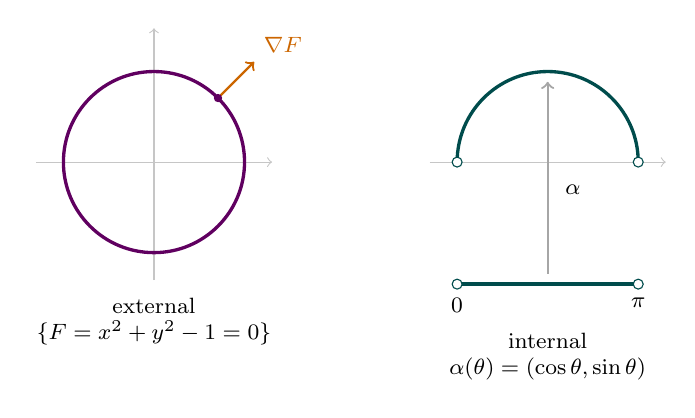
\begin{tikzpicture}[scale=1.0]
\draw[gray!45,->] (-1.5,0)--(1.5,0); \draw[gray!45,->] (0,-1.5)--(0,1.7);
\draw[violet!75!black,very thick] (0,0) circle (1.15);
\draw[orange!80!black,->,thick] (45:1.15) -- (45:1.8);
\node[orange!80!black,font=\footnotesize,anchor=south west] at (45:1.8) {$\nabla F$};
\fill[violet!75!black] (45:1.15) circle (1.5pt);
\node[font=\footnotesize,anchor=north,align=center] at (0,-1.6) {external\\ $\{F=x^2+y^2-1=0\}$};
\begin{scope}[xshift=5.0cm]
\draw[gray!45,->] (-1.5,0)--(1.5,0);
\draw[teal!60!black,very thick] (0:1.15) arc (0:180:1.15);
\draw[teal!60!black, fill=white] (1.15,0) circle (1.8pt); \draw[teal!60!black, fill=white] (-1.15,0) circle (1.8pt);
\draw[teal!60!black,very thick] (-1.15,-1.55) -- (1.15,-1.55);
\draw[teal!60!black, fill=white] (-1.15,-1.55) circle (1.8pt); \draw[teal!60!black, fill=white] (1.15,-1.55) circle (1.8pt);
\node[font=\footnotesize,below] at (-1.15,-1.6) {$0$};
\node[font=\footnotesize,below] at (1.15,-1.6) {$\pi$};
\draw[->,thick,gray!70] (0,-1.42) -- (0,1.02);
\node[font=\footnotesize,anchor=west] at (0.1,-0.35) {$\alpha$};
\node[font=\footnotesize,anchor=north,align=center] at (0,-2.05) {internal\\ $\alpha(\theta)=(\cos\theta,\sin\theta)$};
\end{scope}
\end{tikzpicture}
